%%%%%%%%%%%%%%%%%%%%%%%%%%%%%%%%%%%%%%%%%
% a0poster Portrait Poster
% LaTeX Template
% Version 1.0 (22/06/13)
%
% The a0poster class was created by:
% Gerlinde Kettl and Matthias Weiser (tex@kettl.de)
% 
% This template has been downloaded from:
% http://www.LaTeXTemplates.com
%
% License:
% CC BY-NC-SA 3.0 (http://creativecommons.org/licenses/by-nc-sa/3.0/)
%
%%%%%%%%%%%%%%%%%%%%%%%%%%%%%%%%%%%%%%%%%

%----------------------------------------------------------------------------------------
%	PACKAGES AND OTHER DOCUMENT CONFIGURATIONS
%----------------------------------------------------------------------------------------

\documentclass[a0,portrait]{a0poster}
%\setlength{\paperwidth}{80cm}
%\setlength{\paperheight}{180cm}

\usepackage{multicol} % This is so we can have multiple columns of text side-by-side
\columnsep=100pt % This is the amount of white space between the columns in the poster
\columnseprule=3pt % This is the thickness of the black line between the columns in the poster

\usepackage[svgnames]{xcolor} % Specify colors by their 'svgnames', for a full list of all colors available see here: http://www.latextemplates.com/svgnames-colors

\usepackage{times} % Use the times font
%\usepackage{palatino} % Uncomment to use the Palatino font

\usepackage{graphicx} % Required for including images
%\graphicspath{{figures/}} % Location of the graphics files
\usepackage{booktabs} % Top and bottom rules for table
\usepackage[font=small,labelfont=bf]{caption} % Required for specifying captions to tables and figures
\usepackage{amsfonts, amsmath, amsthm, amssymb} % For math fonts, symbols and environments
\usepackage{wrapfig} % Allows wrapping text around tables and figures
\begin{document}

%----------------------------------------------------------------------------------------
%	POSTER HEADER 
%----------------------------------------------------------------------------------------

% The header is divided into two boxes:
% The first is 75% wide and houses the title, subtitle, names, university/organization and contact information
% The second is 25% wide and houses a logo for your university/organization or a photo of you
% The widths of these boxes can be easily edited to accommodate your content as you see fit

\begin{minipage}[b]{.8\linewidth}
\Huge \color{NavyBlue} \textbf{deSPI: efficient classification of metagenomics reads with lightweight de Bruijn graph-based reference indexing} \color{Black}\\ % Title
%\Huge\textit{An Explora}\\[2cm] % Subtitle
\\
\huge \textbf{Dengfeng Guan \& Bo Liu \& Yadong Wang}\\[0.5cm] % Author(s)
\huge Dept. of Computer Science and Technology, Harbin Institute of Technology\\[0.4cm] % University/organization
\Large \texttt{dfguan@hit.edu.cn}\\
\end{minipage}
%
%\begin{minipage}[b]{0.25\linewidth}
%\includegraphics[width=20cm]{logo.png}\\
%\end{minipage}

\vspace{1cm} % A bit of extra whitespace between the header and poster content

%----------------------------------------------------------------------------------------

\begin{multicols}{2} % This is how many columns your poster will be broken into, a portrait poster is generally split into 2 columns

%----------------------------------------------------------------------------------------
%	ABSTRACT
%----------------------------------------------------------------------------------------

\color{Navy} % Navy color for the abstract

\begin{abstract}

One of the core problems in metagenomics is the classification of shotgun sequencing reads to identify species present in samples. Many supervised classification tools have been developed recently, but they either consume large memory or large computation time. Herein we propose a new classification method, de Bruijn Graph-based Species Identifier (deSPI), which takes advantage of de Bruijn graph and FM-index data structures and a hierarchical top-down strategy to do classification. The experimental results suggest that deSPI uses much less memory than Clark and Kraken and classifies reads much faster than Centrifuge and Kaiju, while maintaining a comparable sensitivity and accuracy.
\end{abstract}

%----------------------------------------------------------------------------------------
%	INTRODUCTION
%----------------------------------------------------------------------------------------

\color{SaddleBrown} % SaddleBrown color for the introduction

\section*{Introduction}

Metagenomics has become a major technique to study the microbiome over the last decades. It can help to uncover the complexity of a microbial community in a specific environment, analyze correlation between the community with the environment, and discover new microbial species that cannot be cultivated in the laboratory. With the development of next-generation sequencing (NGS) technologies and decrease of sequencing cost, ever larger metagenomics sequencing data sets are being produced. While these give us more opportunities to perform microbiome analysis, they also generate many analytical challenges. One of the major computational challenges is metagenomics classification. 

In recent years, numerious supervised metagenomics classification tools that scale efficiently while maintaining sensitivity are developed. Many of them are based on short exact matches. Among these tools, Kraken \cite{Wood2014-es}, Clark \cite{Ounit2015-fi}, Centrifuge \cite{Kim2016-zf}, Kaiju \cite{Menzel2016-mi}, are now being widely used in metagenomics classification. However they either require large memory,  or have low efficiency is relatively low. Herein, we propose deSPI, a novel short exact match based metagenomic read classification tool, which has higher speed and affordable memory cost with higher or comparable sensitivity and accuracy. 

%----------------------------------------------------------------------------------------
%	OBJECTIVES
%----------------------------------------------------------------------------------------

\color{DarkSlateGray} % DarkSlateGray color for the rest of the content

%\section*{Main Objectives}
%
%\begin{enumerate}
%\item Lorem ipsum dolor sit amet, consectetur.
%\item Nullam at mi nisl. Vestibulum est purus, ultricies cursus volutpat sit amet, vestibulum eu.
%\item Praesent tortor libero, vulputate quis elementum a, iaculis.
%\item Phasellus a quam mauris, non varius mauris. Fusce tristique, enim tempor varius porta, elit purus commodo velit, pretium mattis ligula nisl nec ante.
%\item Ut adipiscing accumsan sapien, sit amet pretium.
%\item Estibulum est purus, ultricies cursus volutpat
%\item Nullam at mi nisl. Vestibulum est purus, ultricies cursus volutpat sit amet, vestibulum eu.
%\item Praesent tortor libero, vulputate quis elementum a, iaculis.
%\end{enumerate}

%----------------------------------------------------------------------------------------
%	MATERIALS AND METHODS
%----------------------------------------------------------------------------------------

\section*{Methods}

\begin{center}\vspace{1cm}
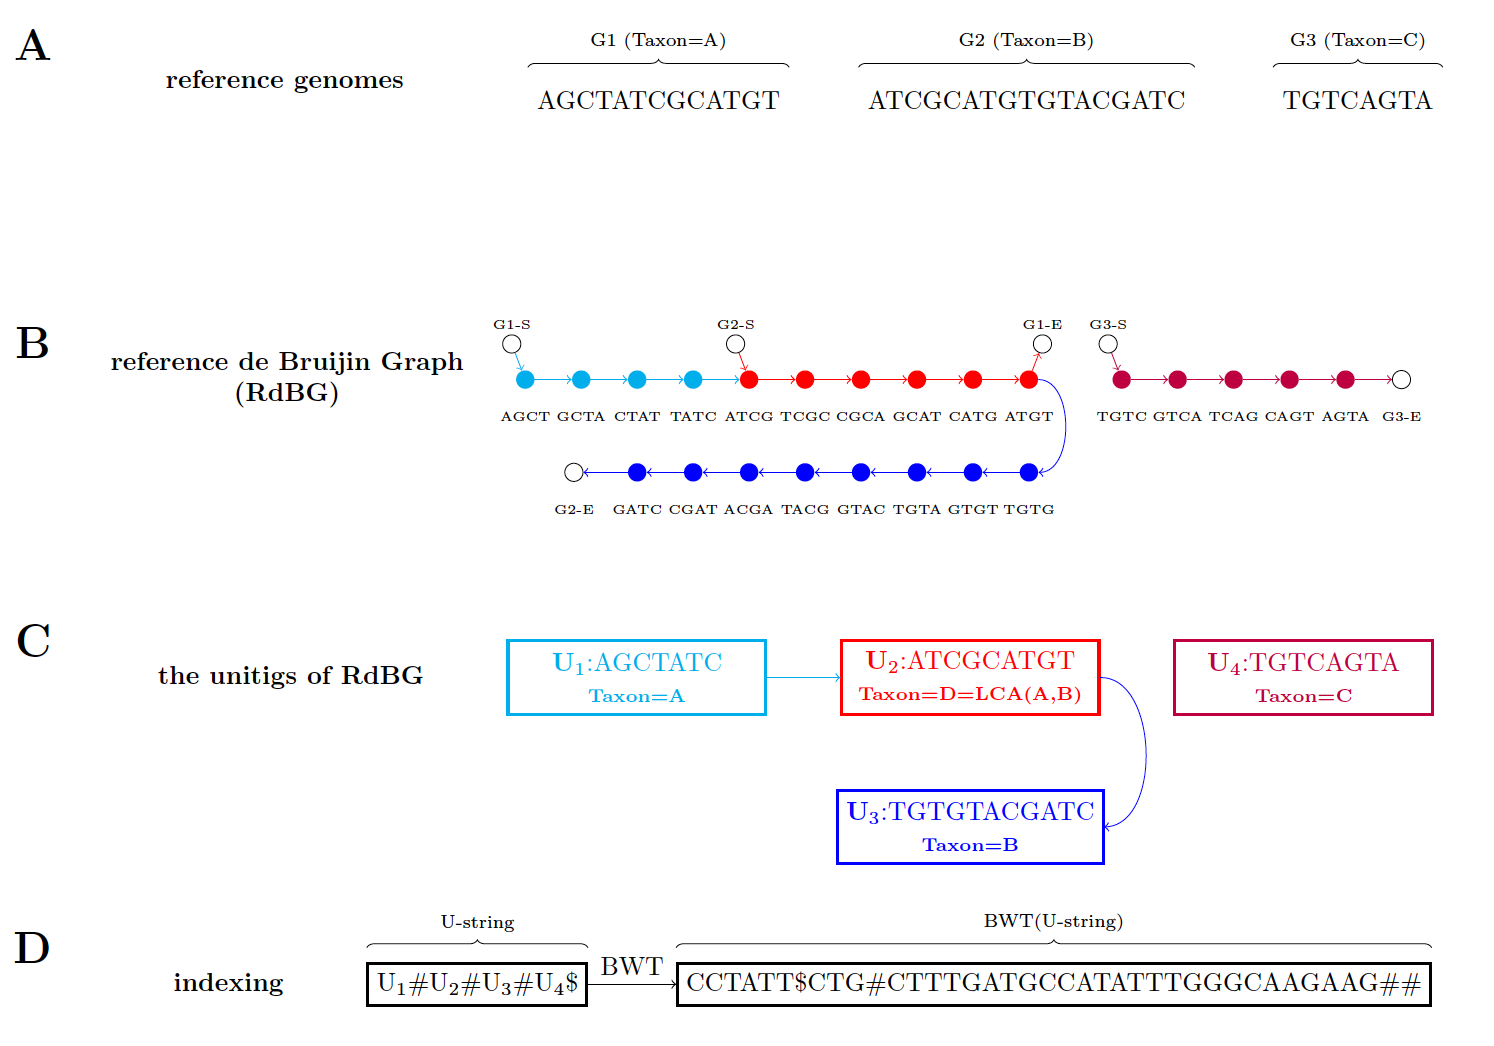
\includegraphics[width=0.7\linewidth]{irg1}
\captionof{figure}{\color{Green} Index Reference Genomes. (\textbf{A}) A library of reference genomes. (\textbf{B}) Build de Bruijn Graph (RdBG) of the reference database. (\textbf{C}) Obtain unitigs from RdBG, each unitig is labeled with a LCA of the organisms containing the unitig. (\textbf{D}) Obtain U-string through joining all unitigs together with a delimiter \#, perform Burrow-Wheeler Transformation on U-string and generate FM-index. }
\end{center}\vspace{1cm}

\begin{center}\vspace{1cm}
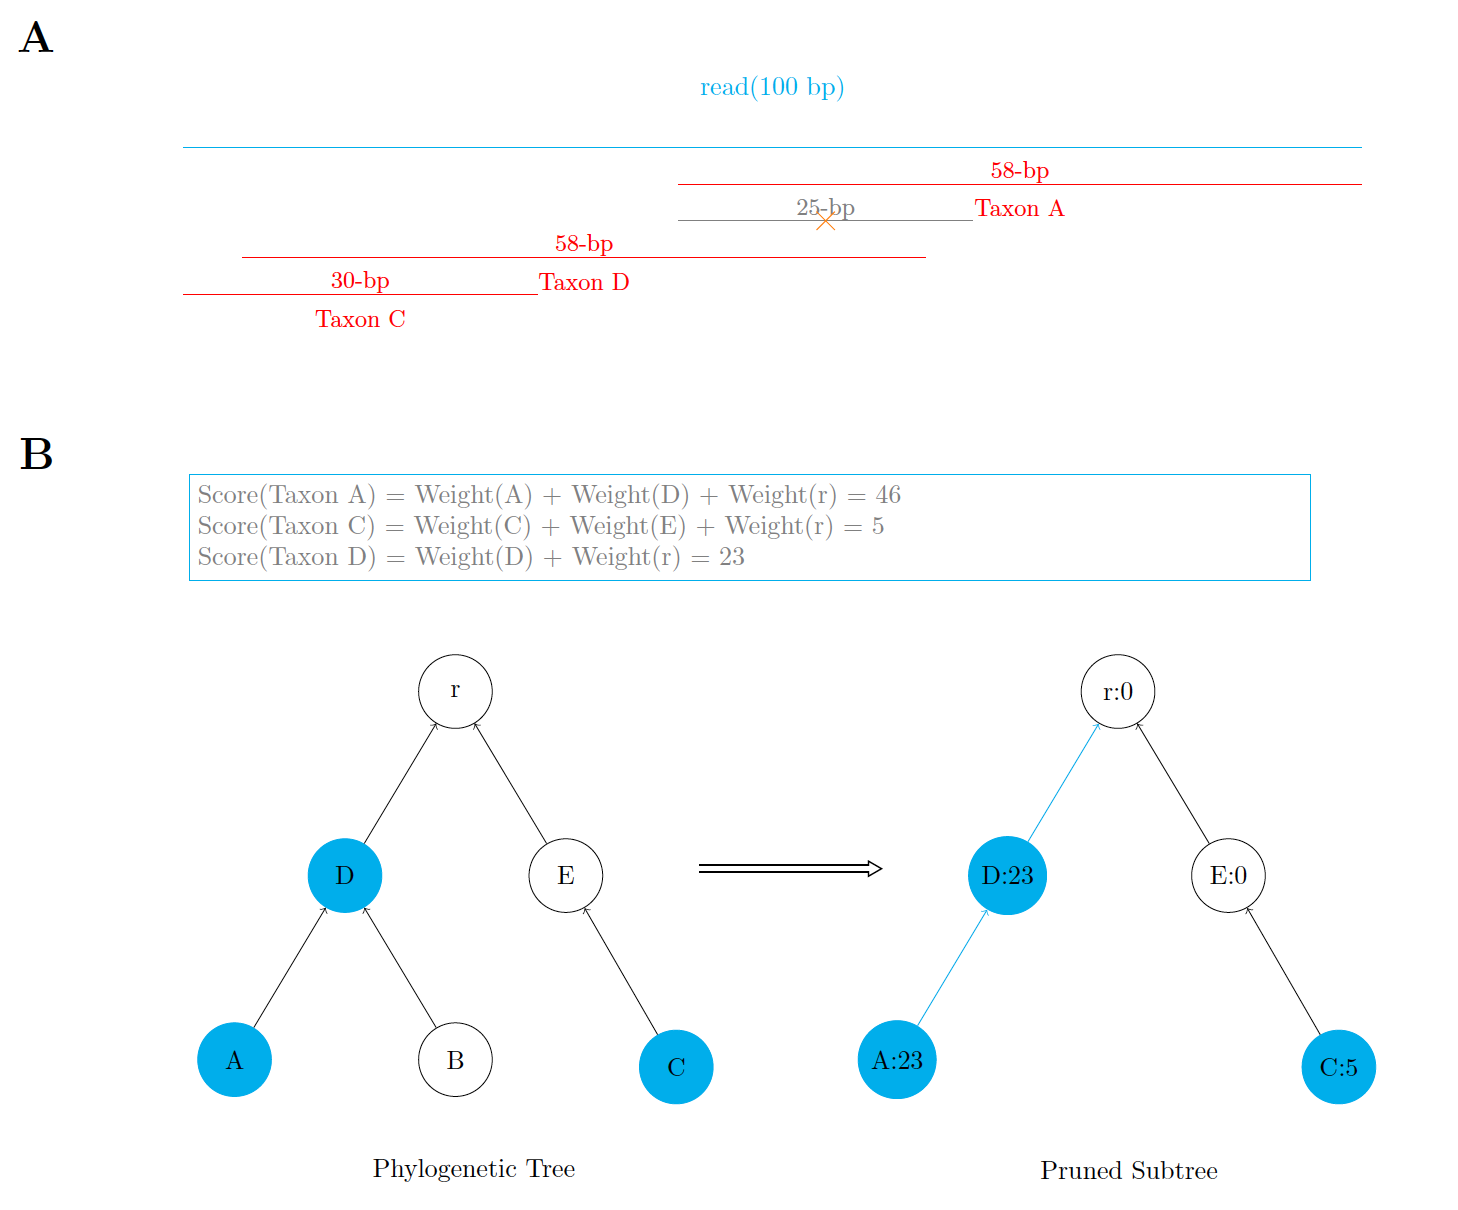
\includegraphics[width=0.7\linewidth]{cor1}
\captionof{figure}{\color{Green} Classification of a read. The figure illustrates the deSPI classification algorithm using seed length 25. (\textbf{A}) deSPI performs backward search along the read, find all U-MEMs larger than the minimum seed length. (\textbf{B}) Nodes receiving hits (highlighted in cyan) form a pruned phylogenetic tree, deSPI traverses the tree to figure out the classification path (nodes and edges highlighted in cyan).}
\end{center}\vspace{1cm}
%Fusce magna risus, molestie ut porttitor in, consectetur sed mi. Vestibulum ante ipsum primis in faucibus orci luctus et ultrices posuere cubilia Curae; Pellentesque consectetur blandit pellentesque. Sed odio justo, viverra nec porttitor vel, lacinia a nunc. Suspendisse pulvinar euismod arcu, sit amet accumsan enim fermentum quis. In id mauris ut dui feugiat egestas. Vestibulum ac turpis lacinia nisl commodo sagittis eget sit amet sapien.






%------------------------------------------------

%\subsection*{Mathematical Section}
%
%Nulla vel nisl sed mauris auctor mollis non sed. 
%
%\begin{equation}
%E = mc^{2}
%\label{eqn:Einstein}
%\end{equation}
%
%Curabitur mi sem, pulvinar quis aliquam rutrum. (1) edf (2)
%, $\Omega=[-1,1]^3$, maecenas leo est, ornare at. $z=-1$ edf $z=1$ sed interdum felis dapibus sem. $x$ set $y$ ytruem. 
%Turpis $j$ amet accumsan enim $y$-lacina; 
%ref $k$-viverra nec porttitor $x$-lacina. 
%
%Vestibulum ac diam a odio tempus congue. Vivamus id enim nisi:
%
%\begin{eqnarray}
%\cos\bar{\phi}_k Q_{j,k+1,t} + Q_{j,k+1,x}+\frac{\sin^2\bar{\phi}_k}{T\cos\bar{\phi}_k} Q_{j,k+1} &=&\nonumber\\ 
%-\cos\phi_k Q_{j,k,t} + Q_{j,k,x}-\frac{\sin^2\phi_k}{T\cos\phi_k} Q_{j,k}\label{edgek}
%\end{eqnarray}
%and
%\begin{eqnarray}
%\cos\bar{\phi}_j Q_{j+1,k,t} + Q_{j+1,k,y}+\frac{\sin^2\bar{\phi}_j}{T\cos\bar{\phi}_j} Q_{j+1,k}&=&\nonumber \\
%-\cos\phi_j Q_{j,k,t} + Q_{j,k,y}-\frac{\sin^2\phi_j}{T\cos\phi_j} Q_{j,k}.\label{edgej}
%\end{eqnarray} 
%
%Nulla sed arcu arcu. Duis et ante gravida orci venenatis tincidunt. Fusce vitae lacinia metus. Pellentesque habitant morbi. $\mathbf{A}\underline{\xi}=\underline{\beta}$ Vim $\underline{\xi}$ enum nidi $3(P+2)^{2}$ lacina. Id feugain $\mathbf{A}$ nun quis; magno.

%----------------------------------------------------------------------------------------
%	RESULTS 
%----------------------------------------------------------------------------------------

\section*{Results}
Three experiments were carried out on simulated and real datasets, to assess the feasibility of deSPI. Four state-of-the-art metagenomics classification tools, Centrifuge, Clark, Kaiju and Kraken are tested on the same datasets for comparison. The \textit{k-mer} used for indices of Clark and Kraken, and RdBG of deSPI is 31. deSPI was tested with seed lengths of 24, 28 and 31, while the other tools were ran with their default settings. For simulated data and real sequencing data from single individuals, the test were run on a server with 1TB of Random Access Memory (RAM), eight 2.0 GHZ Intel Xeon E7-4820 CPUs (64 cores). For the real metagenomic data, the test were performed on a server with 767.8 GB of RAM, fifty-six 2.6 GHZ Intel Xeon E5-2690 CPUs (784 cores). 

\begin{center}\vspace{1cm}
\small
\begin{tabular}{cccccc}
\toprule
& & \textbf{Species} & \textbf{Genus} & \textbf{Memory} & \textbf{Speed} \\
\cline{3-6}
& & Sen/Acc/F1-score & Sen/Acc/F1-score  & GB & Kseq/m \\
\midrule
& 24mer & \textbf{76.59}/96.83/\textbf{85.53} & \textbf{94.28}/99.23/\textbf{96.69} & 25 & 822 \\ 
deSPI & 28mer & 73.64/98.36/84.22 & 91.45/99.54/95.32 & 25 & 853 \\
& 31mer & 70.68/\textbf{99.37}/82.61 & 88.17/\textbf{99.81}/93.63 & 25 & 755 \\
Centrifuge & & 75.06/98.96/85.37 & 91.86/99.71/95.62 & \textbf{10} & 416 \\
Clark & 31mer & 70.54/99.27/82.47 & 70.84/99.69/82.82 & 79 & \textbf{1077} \\
Kaiju & & 40.23/95.56/56.62 & 63.38/98.17/77.03 & 14 & 195 \\
Kraken & 31mer & 71.83/99.26/83.34 & 89.39/99.78/94.30 & 126 & 722 \\
\bottomrule
\end{tabular}
\captionof{table}{\color{Green} Classification performance for deSPI, Centrifuge, Clark, Kaiju and Kraken on simulated reads}
\end{center}\vspace{1cm}

\begin{center}\vspace{1cm}
\footnotesize
\begin{tabular}{ccccc|ccc|c}
\toprule
& & & \textbf{HiSeq Single-end} & && \textbf{MiSeq Single-end} & & \\
%\cline{3-5}\cline{6-8}
& & \textbf{Species} & \textbf{Genus} & \textbf{Speed} & \textbf{Species} & \textbf{Genus} & \textbf{Speed} & \textbf{Memory}\\
\cline{3-5}\cline{6-9}
& & Sen/Acc/F1-score & Sen/Acc/F1-score & Kseq/m &Sen/Acc/F1-score & Sen/Acc/F1-score & Kseq/m & GB\\
\midrule
& 24mer &\textbf{34.46}/94.98/\textbf{50.57} & \textbf{49.05}/97.55/\textbf{65.28} & 1562 & \textbf{21.45}/68.76/\textbf{32.70} & \textbf{56.36}/95.86/\textbf{70.99} & 1004 & 25 \\
deSPI & 28mer & 34.11/96.70/50.43 & 47.91/98.36/64.43 & 1600& 21.05/72.25/32.60 & 55.33/96.92/70.45 & 993& 25\\
 & 31mer & 33.80/\textbf{97.44}/50.19 & 46.86/\textbf{98.69}/63.55 & 1580 & 20.79/74.19/32.48 & 54.64/\textbf{97.36}/70.00 & 969 & 25\\
Centrifuge	 & & 34.20/93.72/50.11 & 48.21/97.89/64.60 & 715 &20.85/68.81/32.00 & 55.00/96.29/70.01 & 453 & \textbf{10}\\
Clark & 31mer & 33.74/97.20/50.09 & 34.02/98.02/50.51 & \textbf{2060} & 20.74/\textbf{74.56}/32.45 & 26.43/95.01/41.35 & \textbf{1074} & 79 \\
Kaiju	 & & 19.09/91.18/31.57 & 30.11/95.44/45.78 & 262 & 9.21/62.14/16.04 & 42.85/94.18/58.90 & 231 & 14\\
Kraken & 31mer & 33.89/97.32/50.27 & 47.29/98.66/63.93 & 1143 & 20.89/73.70/32.55 & 54.92/97.27/70.20 & 873 & 126\\
\bottomrule 
\end{tabular}
\captionof{table}{\color{Green} Classification performance of all tools on single-end datasets}
\end{center}\vspace{1cm}

\begin{center}\vspace{1cm}
\footnotesize
\begin{tabular}{ccccc|ccc|c}
\toprule
& & & \textbf{HiSeq Paired-End} & && \textbf{MiSeq Paired-End} & & \\
%\cline{3-5}\cline{6-8}
& & \textbf{Species} & \textbf{Genus} & \textbf{Speed} & \textbf{Species} & \textbf{Genus} & \textbf{Speed} & \textbf{Memory}\\
\cline{3-5}\cline{6-9}
& & Sen/Acc/F1-score & Sen/Acc/F1-score & Kseq/m &Sen/Acc/F1-score & Sen/Acc/F1-score & Kseq/m & GB\\
\midrule
& 24mer & \textbf{35.04}/52.00/41.87 & \textbf{69.29}/88.76/\textbf{77.83} & 537 &\textbf{74.10}/82.20/77.94 & \textbf{89.94}/96.13/\textbf{92.93} & 246& 25\\
deSPI & 28mer & 34.43/55.16/42.39 & 67.68/91.37/77.76 & 544 &73.73/83.77/78.43 & 89.08/97.12/92.93 & 230 & 25\\
& 31mer & 33.94/\textbf{56.76}/42.48 & 66.50/\textbf{92.34}/77.32 & 526 & 73.39/\textbf{84.59}/\textbf{78.59} & 88.44/\textbf{97.53}/92.76 & 201 & 25\\
Centrifuge && 34.39/54.19/42.08 & 67.89/89.65/77.27 & 365 &72.77/83.07/77.58 & 87.86/96.48/91.97 & 107 & \textbf{10} \\
Clark & 31mer & 33.90/57.23/\textbf{42.58} & 53.63/90.57/67.37 & \textbf{689} & 73.34/84.40/78.48 & 84.46/97.21/90.39 & \textbf{298} & 79\\
Kaiju && 21.69/47.68/29.82 & 55.64/85.83/67.51 & 175  & 32.21/72.08/44.53 & 50.80/93.51/65.84 & 105 & 14\\
Kraken & 31mer & 34.09/56.24/42.45 & 66.92/91.96/77.47 & 454 & 73.44/84.35/78.52 & 88.63/97.42/92.82 & 213 & 126 \\
\bottomrule
\end{tabular}
\captionof{table}{\color{Green} Classification performance of all tools on paired-end datasets}
\end{center}\vspace{1cm}

\begin{center}\vspace{1cm}
\footnotesize
\begin{tabular}{ccccc}
\toprule
& & \textbf{Species} & \textbf{Memory} & \textbf{Speed}\\
\cline{3-5}
& & Sen/Acc/F1-score & GB & KSeq/m\\
\midrule
%deSPI & 24mer & 34.16/76.91/47.31 & 34.16/72.82/46.51 \\
%Centrifuge	 & & 34.51/72.10/46.68 & 34.51/68.43/45.88\\
%Clark	 & 31mer & 24.57/96.57/39.17 & 24.57/85.75/38.19\\
%Kaiju	 & & 48.97/35.86/41.40 & 48.97/39.72/43.87 \\
%Kraken & 31mer & 27.93/86.75/42.25 & 27.93/81.85/41.65\\
deSPI & 24mer & 34.16/76.91/\textbf{47.31} & 25 & 1025\\
Centrifuge	 & & 34.51/72.10/46.68 & \textbf{9} & 971\\
Clark	 & 31mer & 24.57/\textbf{96.57}/39.17 & 70 & 1630\\
Kaiju	 & & \textbf{48.97}/35.86/41.40 & 14 & 319\\
Kraken & 31mer & 27.93/86.75/42.25 & 126 & \textbf{1673}\\
\bottomrule
\end{tabular}
\captionof{table}{\color{Green} Classification performance of all tools on real metagenomics datasets}
\end{center}\vspace{1cm}
%Donec faucibus purus at tortor egestas eu fermentum dolor facilisis. Maecenas tempor dui eu neque fringilla rutrum. Mauris \emph{lobortis} nisl accumsan. Aenean vitae risus ante.
%
%\begin{wraptable}{l}{12cm} % Left or right alignment is specified in the first bracket, the width of the table is in the second
%\begin{tabular}{l l l}
%\toprule
%\textbf{Treatments} & \textbf{Response 1} & \textbf{Response 2}\\
%\midrule
%Treatment 1 & 0.0003262 & 0.562 \\
%Treatment 2 & 0.0015681 & 0.910 \\
%Treatment 3 & 0.0009271 & 0.296 \\
%\bottomrule
%\end{tabular}
%\captionof{table}{\color{Green} Table caption}
%\end{wraptable}
%%
%Phasellus imperdiet, tortor vitae congue bibendum, felis enim sagittis lorem, et volutpat ante orci sagittis mi. Morbi rutrum laoreet semper. Morbi accumsan enim nec tortor consectetur non commodo nisi sollicitudin. Proin sollicitudin. Pellentesque eget orci eros. Fusce ultricies, tellus et pellentesque fringilla, ante massa luctus libero, quis tristique purus urna nec nibh.
%
%Nulla ut porttitor enim. Suspendisse venenatis dui eget eros gravida tempor. Mauris feugiat elit et augue placerat ultrices. Morbi accumsan enim nec tortor consectetur non commodo. Pellentesque condimentum dui. Etiam sagittis purus non tellus tempor volutpat. Donec et dui non massa tristique adipiscing. Quisque vestibulum eros eu. Phasellus imperdiet, tortor vitae congue bibendum, felis enim sagittis lorem, et volutpat ante orci sagittis mi. Morbi rutrum laoreet semper. Morbi accumsan enim nec tortor consectetur non commodo nisi sollicitudin.

%\begin{center}\vspace{1cm}
%\includegraphics[width=0.8\linewidth]{placeholder}
%\captionof{figure}{\color{Green} Figure caption}
%\end{center}\vspace{1cm}
%
%In hac habitasse platea dictumst. Etiam placerat, risus ac.
%
%Adipiscing lectus in magna blandit:
%
%\begin{center}\vspace{1cm}
%\begin{tabular}{l l l l}
%\toprule
%\textbf{Treatments} & \textbf{Response 1} & \textbf{Response 2} \\
%\midrule
%Treatment 1 & 0.0003262 & 0.562 \\
%Treatment 2 & 0.0015681 & 0.910 \\
%Treatment 3 & 0.0009271 & 0.296 \\
%\bottomrule
%\end{tabular}
%\captionof{table}{\color{Green} Table caption}
%\end{center}\vspace{1cm}
%
%Vivamus sed nibh ac metus tristique tristique a vitae ante. Sed lobortis mi ut arcu fringilla et adipiscing ligula rutrum. Aenean turpis velit, placerat eget tincidunt nec, ornare in nisl. In placerat.
%
%\begin{center}\vspace{1cm}
%\includegraphics[width=0.8\linewidth]{placeholder}
%\captionof{figure}{\color{Green} Figure caption}
%\end{center}\vspace{1cm}

%----------------------------------------------------------------------------------------
%	CONCLUSIONS
%----------------------------------------------------------------------------------------

\color{SaddleBrown} % SaddleBrown color for the conclusions to make them stand out

\section*{Conclusions}
Herein, we propose a novel algorithm, deSPI, for the classification of metagenomics reads. deSPI indexes unitigs of a de Bruijn graph of a reference database with FM-index, and performs top-down hierarchical taxonomic classification to infer the reads' label. One of the advantages of deSPI is that, with its innovative genome indexing approach, it can use several folds smaller RAM space than \textit{k-mer} index based approaches like Kraken and Clark, to achieve similar speed, which is faster than other proposed approaches using small size index, e.g., Centrifuge and Kaiju. As the memory footprint is only around 25 GB when using all RefSeq complete genome sequences as reference, deSPI can fit to the configurations of most modern PCs and workstations. Moreover, the classification results on hundreds of simulated and real sequencing datasets demonstrated that, in most cases, deSPI can achieve overall the best classification results (F1-score), and its accuracy is also comparable to (if not higher than) state-of-the-art approaches. Considering its lightweight, fast speed and relatively good classification ability, we believe deSPI can have enormous potential to be applied in metagenomics data analysis. 

%\begin{itemize}
%\item Pellentesque eget orci eros. Fusce ultricies, tellus et pellentesque fringilla, ante massa luctus libero, quis tristique purus urna nec nibh. Phasellus fermentum rutrum elementum. Nam quis justo lectus.
%\item Vestibulum sem ante, hendrerit a gravida ac, blandit quis magna.
%\item Donec sem metus, facilisis at condimentum eget, vehicula ut massa. Morbi consequat, diam sed convallis tincidunt, arcu nunc.
%\item Nunc at convallis urna. isus ante. Pellentesque condimentum dui. Etiam sagittis purus non tellus tempor volutpat. Donec et dui non massa tristique adipiscing.
%\end{itemize}

\color{DarkSlateGray} % Set the color back to DarkSlateGray for the rest of the content

%----------------------------------------------------------------------------------------
%	FORTHCOMING RESEARCH
%----------------------------------------------------------------------------------------

%\section*{Forthcoming Research}
%
%Vivamus molestie, risus tempor vehicula mattis, libero arcu volutpat purus, sed blandit sem nibh eget turpis. Maecenas rutrum dui blandit lorem vulputate gravida. Praesent venenatis mi vel lorem tempor at varius diam sagittis. Nam eu leo id turpis interdum luctus a sed augue. Nam tellus.

 %----------------------------------------------------------------------------------------
%	REFERENCES
%----------------------------------------------------------------------------------------

%\nocite{*} % Print all references regardless of whether they were cited in the poster or not
\bibliographystyle{plain} % Plain referencing style
\bibliography{deSPI-refs.bib} % Use the example bibliography file sample.bib

%----------------------------------------------------------------------------------------
%	ACKNOWLEDGEMENTS
%----------------------------------------------------------------------------------------

\section*{Acknowledgements}

This work has been supported by the National Key Research and Development Program of China (No. 2018YFC0910504 and No. 2017YFC0907500), and China Scholarship Council. And we thank Richard Durbin for comments on the manuscript.

%----------------------------------------------------------------------------------------

\end{multicols}
\end{document}